\chapter{Étude statistique des algorithmes de résolution}\label{annexe_stats}
Le module \texttt{bn\_stats.py} fournit, dans la classe \texttt{Stats}, les outils pour analyser statistiquement une distribution de valeurs (calculs des indicateurs statistiques classiques, représentation en histogramme et diagramme en boîte grâce aux modules \texttt{numpy} et \texttt{matplotlib}).

Cette classe fournit également les outils pour sauvegarder et charger la liste des résultats bruts dans un fichier texte pour des analyses plus poussées futures.
\section{Niveau 5}
Les résultats obtenues sur un échantillon de $n=1\,000\,000$ parties sont les suivants :
\begin{center}
\begin{tabular}[t]{|c|l|}
\hline
Nombre de coups & Effectifs\\
\hline
21 & 5\\
\hline
22 & 12\\
\hline
23 & 38\\
\hline
24 & 139\\
\hline
25 & 345\\
\hline
26 & 756\\
\hline
27 & 1635\\
\hline
28 & 3141\\
\hline
29 & 5188\\
\hline
30 & 8244\\
\hline
31 & 12579\\
\hline
32 & 17849\\
\hline
33 & 24091\\
\hline
34 & 30884\\
\hline
35 & 38162\\
\hline
36 & 45397\\
\hline
37 & 51988\\
\hline
38 & 57489\\
\hline
39 & 61778\\
\hline
40 & 64082\\
\hline
41 & 64215\\
\hline
42 & 62822\\
\hline
43 & 59966\\
\hline
\end{tabular}\hspace{0.5cm}
\begin{tabular}[t]{|c|l|}
\hline
Nombre de coups & Effectifs\\
\hline
44 & 56471\\
\hline
45 & 51981\\
\hline
46 & 46666\\
\hline
47 & 41422\\
\hline
48 & 35961\\
\hline
49 & 31474\\
\hline
50 & 26963\\
\hline
51 & 22700\\
\hline
52 & 19270\\
\hline
53 & 15816\\
\hline
54 & 12374\\
\hline
55 & 9586\\
\hline
56 & 6861\\
\hline
57 & 4819\\
\hline
58 & 3020\\
\hline
59 & 1844\\
\hline
60 & 1062\\
\hline
61 & 521\\
\hline
62 & 241\\
\hline
63 & 101\\
\hline
64 & 28\\
\hline
65 & 10\\
\hline
66 & 4\\
\hline
\end{tabular}
\end{center}

\begin{center}\label{histo_algo}
\fbox{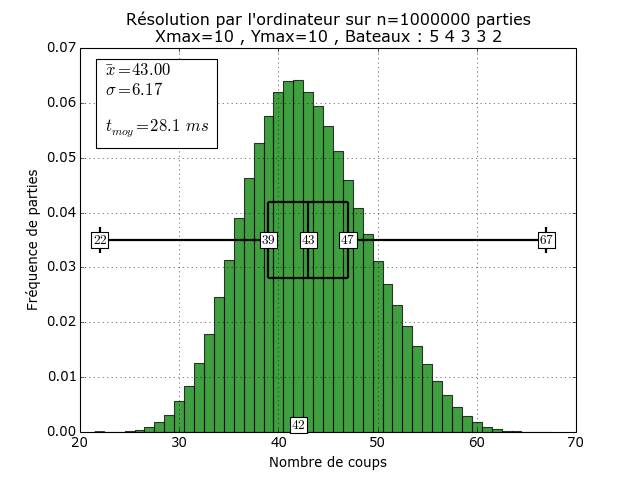
\includegraphics[scale=0.7]{./media/distrib_1000000.png}}
\end{center}

Notons les excellentes performances avec une moyenne de 42,06 coups pour un temps de résolution moyen de seulement 31,2 ms\footnote{Temps mesuré sur un processeur Intel Core i7 4800-MQ à 2,7 Ghz} par partie.
